\documentclass[aps,prl,twocolumn,superscriptaddress,nofootinbib]{revtex4-1}

% the percent sign gives comments in Latex
% top line indicates this is for Physical Review, standard journal format,
% suitable for electronic submission of articles

% the line above is necessary to start any latex document.
% this is one variation that should work for most things.
% if you want double spaceing, use the following:
%
%\documentclass[prd,preprint,letterpaper]{revtex4}
%
% the "preprint" designation will make a wider line
% spacing, good for markup.
\usepackage{graphicx}  % this is the up-to-date package for all figures
\usepackage{amssymb}   % for math
\usepackage{verbatim}  % for the comment environment
\usepackage{color}
\usepackage{gensymb}
\usepackage{amsmath}

\usepackage[section]{placeins}

\usepackage{wrapfig}
\usepackage{hyperref}
\usepackage{titlesec}
\usepackage{amssymb}   % for math
\usepackage{verbatim}  % for the comment environment
\usepackage{color}
\usepackage[nodisplayskipstretch]{setspace}
\usepackage{amsmath}
\usepackage{blindtext}
%\usepackage[pdftex]{graphicx}
\usepackage[outdir=./]{epstopdf}
\usepackage[space]{grffile}
\usepackage{epsfig}
\usepackage[separate-uncertainty=true]{siunitx}
\usepackage{tikz}
\usepackage{pgfgantt}
\usepackage[english]{babel}
\usepackage[utf8]{inputenc}

\titlespacing*{\section}
{0pt}{.5\baselineskip}{.5\baselineskip}

\titlespacing*{\subsection}
{0pt}{.5\baselineskip}{.3\baselineskip}

\usepackage{footnote}

\bibliographystyle{apsrev}


% these are some custom control of the page size and margins
% \topmargin= 0.2in  % these 1st two may be needed for some computers
% \textheight=8.75in
%\textwidth=6.5in
%\oddsidemargin=0cm
%\evensidemargin=0cm

% this is where the actual document itself (rather than control statements) begins:

\begin{document}

% use a style that gives automatic headings
%\pagestyle{headings}



% the \title{} command generates a title.

% the \\ below is used to FORCE a line break in the middle of the sentence--
% otherwise latex computes it for you

\title{Measurements of Polarization Phenomena}


\author{\textbf{Bryan Yamashiro}}
\author{Christina Nelson}
\author{Corey Mutnik}
\author{Daichi Hiramatsu}

\affiliation{Department of Physics \& Astronomy, \\
University of Hawaii at Manoa,\\
2505 Correa Rd, Honolulu, HI, 96822, USA}





	      % \section is used to start a new one with a heading
\begin{abstract}

The experiment involved measuring polarization phenomena including the Brewster angle, extinction ratio for polarized light\,(Malus's Law) and birefringence of a custom sapphire crystal\,\cite{1}. The Brewster angle for BK7 was 303.5\degree$\pm$0.08\degree and the calculated index of refraction was 1.5112$\pm$0.0046. For dielectric and metal mirrors used in this study, the phase shift was 20.90\degree$\pm$0.12\degree. Maximum and minimum intensity values from the Malus's law plot were 9.96\,V$\pm$0.02\,V and 0.02\,V$\pm$0.01\,V respectively. Using the two intensity values, the extinction ratio was 456.40$\pm$210.69. The difference between the two angles is 89.95\degree$\pm$0.14\degree, with a 0.33$\sigma$ deviation. The resulting angle was approximately perpendicular, therefore the experiment verified Malus's Law. The cosine squared fit exhibited a low chi squared. A low chi squared meant that intensities were detected and converted properly into voltages, proving that the diode detector had a linear response. The two $\alpha$ angles for the first and second birefringence minimums of the sapphire crystal were 28.07\degree$\pm$0.04\degree and 27.69\degree$\pm$0.03\degree respectively. The weighted average of the two c-axis values is 28.88\degree$\pm$0.04\degree.

\end{abstract}

\maketitle    % this line is necessary to tell latex you are done with all
	      % of the stuff associated with the title, and now it can go
              % ahead and generate the title portion


\section{Background}

The term polarization refers to a property of light being polarized, but also the production of polarized light\,\cite{2}. The Sun is the main source of light seen on Earth, and the emitted light is unpolarized. The blue sky that we observe is a result of Rayleigh scattering. An application of polarization is reducing reflected light off of surfaces such as the ocean or wet roads. Light is reflected off reflective surfaces and causes large amounts of intense light projected into our eyes. The intense light is polarized by reflection and unpolarized sunlight becomes linearly polarized at defined angles, usually horizontally. Light is a transverse electromagnetic wave and thus it can be polarized. To suppress harsh light reflections one needs a vertical linear polarizer to eliminate the reflected light and to allow propagation of unpolarized light.
\\
\indent Sunlight above the atmosphere is not polarized. This is predicament for cameras mounted on satellites above Earth orbit, and especially near the Lagrange point 1\,(L1). The Solar Dynamics Observatory\,(SDO) is a NASA satellite currently in L1. The SDO is equipped with a coronagraph camera able to study variations in the solar irradiance\,\cite{3}. To obtain images seen in figure \ref{sdo}, polarizers allow limited light into the camera to be converted from the coronagraphs. Polarized images of the Sun allow us to observe powerful and bright solar event propagation with defined structures.

\begin{figure}[h!]
  \begin{center}
\centerline{\includegraphics[width=3.5in]{sdo.jpg}}
\caption{\small{SDO coronagraph images at different wavelengths, polarized visible light to 304\,\AA. \label{sdo}}}
  \end{center}
\end{figure}



 % the ~\cite{ } is how you link a reference in the text. The references
 % themselves are at the end.

% one or more lines of space between paragraphs determines them

\section{Apparatus}


\begin{figure}[h!]
  \begin{center}
\centerline{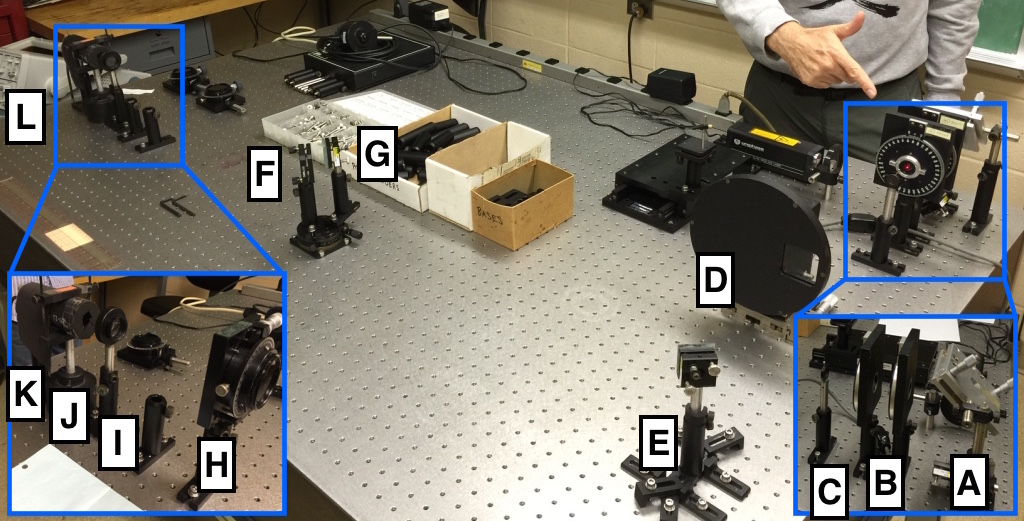
\includegraphics[width=3.5in]{apparatus.jpg}}
\caption{\small{A)\,Laser source B)\,Variable linear polarizer C)\,Iris D)\,Chopper E)\,Mirror F)\,BK7 G)\,Mirror H)\,Lens I)\,Light sheath J)\,Detector K)\,Oscilloscope \label{app1}}}
  \end{center}
\end{figure}
\vspace{-.7cm}
\vfill\eject
The experiment apparatus involved several components in the path of a Helium-Neon\,(HeNe) laser source seen in figure \ref{app1}. The HeNe laser source\,(A) initially passes through a variable linear polarizer\,(B) that can select a vertical, horizontal, or linear state in between. The polarized source is then passed through an iris\,(C) and light chopper\,(D). The iris allows the baseline and signal to be viewed simultaneously on the oscilloscope. From the chopper, the laser is reflected off of an initial mirror\,(E) to the BK7\,(F), reflected off the BK7 to a second mirror\.(G), and from the second mirror to a lens\,(H). The lens ejects a parallel transport to the diode detector\,(J) and a measurement is read off the oscilloscope\,(K). To reduce background light, a sheath\,(I) is placed between the lens and the detector. For the sapphire birefringence procedure, the reflecting array including components\,(F and G), are replaced with the custom sapphire crystal on a rotating pedestal.



\section{Procedure}

This study consisted of observing the polarization phenomena, production and measurements of various states of polarization, polarizing components and systems, and observing the birefringence of sapphire. Using the apparatus in figure \ref{app1}, we measured the Brewster angle and the relative phase shift of linearly polarized light upon reflection from a metal mirror and a dielectric. The next part of the experiment involved manipulating the angle of polarization. The result of varying polarization angles affected the output voltages, which was compared to Malus's Law. Finally, a custom sapphire crystal was used to observe birefringence and the angle of the crystal c-axis. The apparatus (F-G) components, seen in figure \ref{app1}, were replaced with a the custom sapphire crystal at a neutral perpendicular angle. The sapphire crystal was tilted at various angles to measure the minimum amplitude angles clockwise and counterclockwise from the neutral angle perpendicular to the HeNe laser beam.

\vfill\eject



\section{Calculation of Results}
\subsection{Brewster angle measurement}
The index of refraction measured for BK7 is 1.5112$\pm$0.0046. This answer was calculated from the Brewster angle, which is 303.5\degree$\pm$0.08\degree. This value was subtracted from 360\degree resulting in an angle of 56.5\degree. The tangent of the resulting angle was multiplied by the refractive index of air. The experimental index value was compared to the accepted value at the HeNe wavelength, 1.515, which corresponds to a 0.83$\sigma$ deviation.

\subsection{Production and measurement of various states of polarization}
A dielectric and a metal mirror were set to 46\degree and the polarizer was set to 166\degree. We observed that the signal was not completely extinguished meaning there is elliptical polarization.

\begin{equation}
\phi = \cos^{-1}\left(\frac{I_+-I_-}{2\sqrt{I_xI_y}}\right)
\label{phase}
\end{equation}

Values in equation \ref{phase} included the phase angle, $\phi$, and intensities at the angles, -45\degree, 0\degree, 45\degree, and 90\degree. The corresponding angles with respective intensities were I$_x$\,(90\degree), I$_y$\,(0\degree), I$_-$\,(-45\degree), and I$_+$\,(45\degree). Intensities for I$_x$\, I$_y$\, I$_-$, and I$_+$ were 1.45\,V$\pm$0.15\,V, 1.56\,V$\pm$0.16\,V, 2.93\,V$\pm$0.29\,V, and 0.12\,V$\pm$0.01\,V. The measured relative phase shift, $\phi$, is $\pm$20.90\degree$\pm$0.12\degree.

\subsection{Polarizing components and systems}

\begin{figure}[h!]
  \begin{center}
\centerline{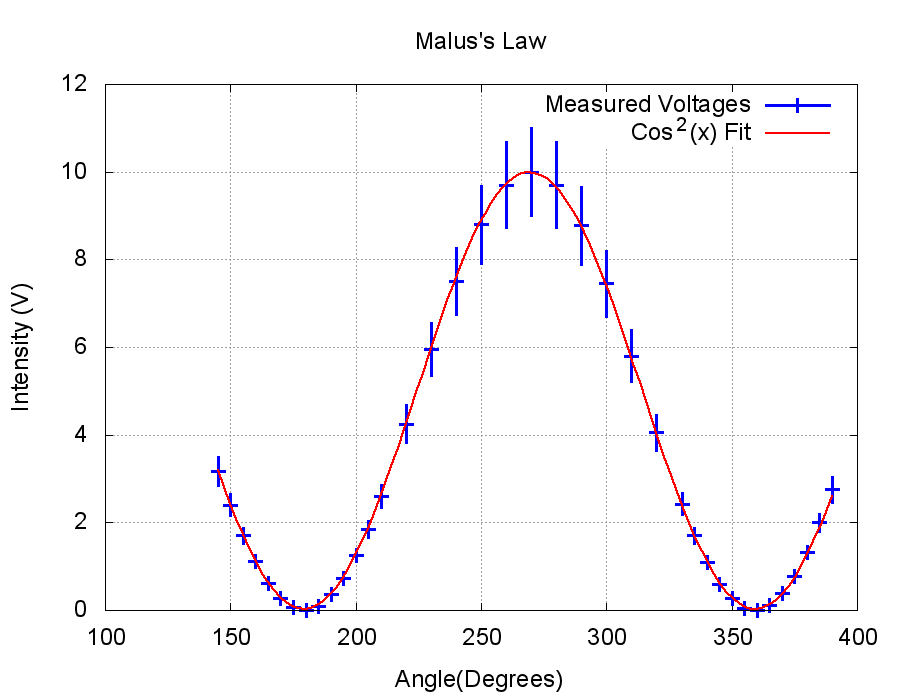
\includegraphics[width=3.5in]{malus.png}}
\caption{\small{Intensities from an initial $<$2\,V angle\,(145\degree) to a final angle at $<$2\,V\,(390\degree). The data in blue is fit with a cosine squared fit. \label{malus}}}
  \end{center}
\end{figure}
\vspace{-.7cm}

\begin{equation}
I=I_0\cos^{2}(\theta-\theta_c)+C
\label{maleqn}
\end{equation}

Equation \ref{maleqn} was used as a fit for our data values. The quantity, $I_0$, is the maximum intensity peak value, $\theta_c$ is the angle of the maximum peak, and C is a constant that is regarded as the minimum intensity value. The cosine squared fit yield maximum and minimum intensity values of 9.96\,V$\pm$0.02\,V and 0.02\,V$\pm$0.01\,V, respectively. Using the two intensity values, the extinction value was determined with the maximum over minimum intensity, which yields 456.40$\pm$210.69. The plotting program determined the reduced chi squared of the fit, $\frac{\chi^2}{ndf}$, to be 0.002. The cosine squared fit showing a relatively low chi squared value meaning that intensities were detected and converted properly into voltages, proving that the diode detector had a linear response.
\\
\indent According to Malus's law, the polarizer will transmit a wave of the largest amplitude at the plane of transmission, conversely, rejecting the relative perpendicular component\,\cite{4}. A cosine squared fit was used to find the maximum amplitude angle, 269.35\degree$\pm$0.07\degree, and a quadratic fit was used to find the minimum amplitude angle, 179.40\degree$\pm$0.07\degree. The difference between the two angles is 89.95\degree$\pm$0.14\degree. With a 0.33$\sigma$ deviation, the resulting angle is perpendicular, therefore the experiment verifies Malus's Law.

\subsection{Birefringence of sapphire}
\begin{figure}[h!]
  \begin{center}
\centerline{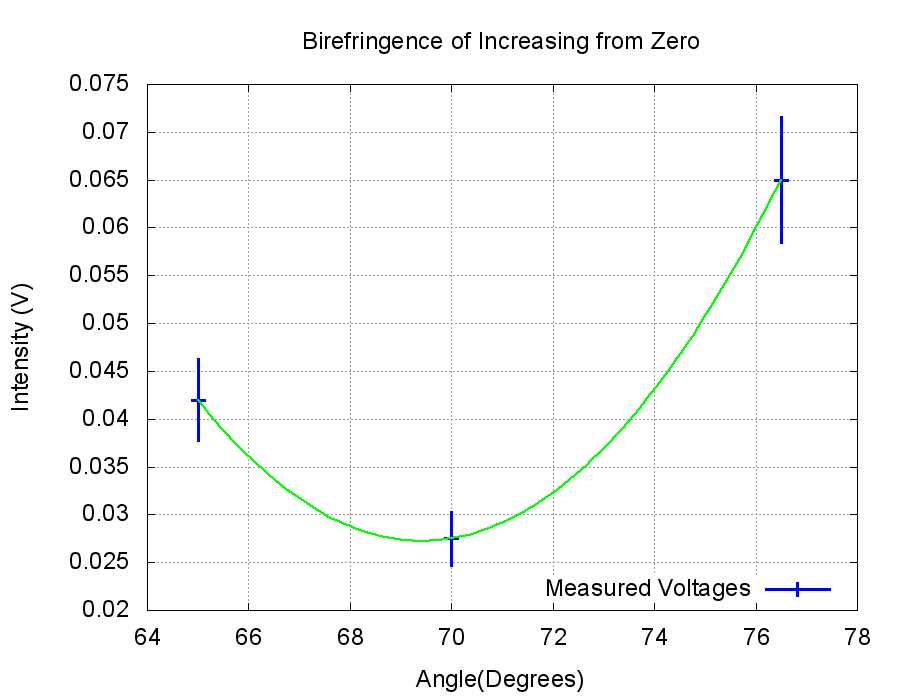
\includegraphics[width=3.5in]{bire1.png}}
\caption{\small{The intensity versus angle for the minimum angles of the polarizer. The intensity include values under 2\,V, and a quadratic function is fit to the points with angles between 65\degree-77\degree. \label{bire1}}}
  \end{center}
\end{figure}
\vspace{-.7cm}

\begin{figure}[h!]
  \begin{center}
\centerline{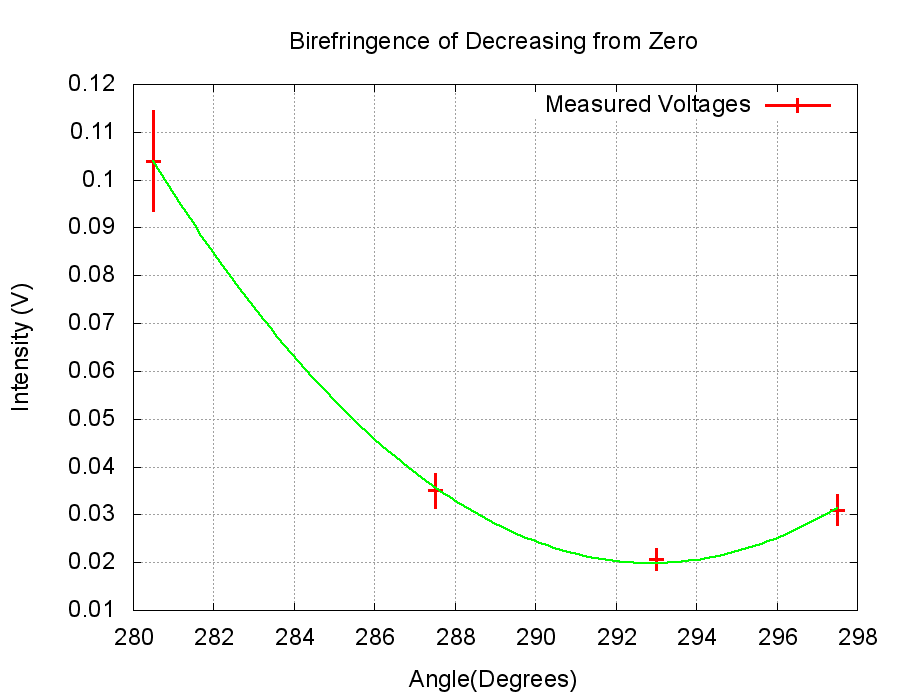
\includegraphics[width=3.5in]{bire2.png}}
\caption{\small{The intensity versus angle for the minimum angles of the polarizer. The intensity include values under 2\,V, and a quadratic function is fit to the points with angles between 280\degree-300\degree. \label{bire2}}}
  \end{center}
\end{figure}
\vspace{.7cm}

Figures \ref{bire1} and \ref{bire2} both yielded minimum amplitude angles of the sapphire crystal. Both figures show intensity versus angles and were fit with quadratic equations. The first birefringence minimum angle, $\theta$$_1$ between angles 65\degree-77\degree is 69.40\degree$\pm$0.20\degree. The second birefringence minimum angle, $\theta$$_2$, between angles 280\degree-300\degree is 292.90\degree$\pm$0.17\degree. Figure \ref{bire1} showed three points, and since we use a second degree polynomial that fits with three parameters.

\begin{equation}
\alpha=\tan^{-1}\left(\frac{n_{air}\sin(\theta_3)}{n_e}\right)
\label{snell}
\end{equation}

Equation \ref{snell} was derived from Snell's law and a provided equation for a full 90\degree rotation for the apex angle, $\alpha$. The apex angle represents the maximum amplitude peak, similar to the Malus's law in figure \ref{malus}. The two figures \ref{bire1} and \ref{bire2} are the two minimums, and the apex angle is where the major amplitude peak lies. The equation includes the constants n$_{air}$=1.000293 and n$_e$=1.756. The two minimum angle values, $\theta$$_1$ and $\theta$$_2$, were substituted for $\theta_3$.
\\
\indent The two $\alpha$ angles for the first and second birefringence minimums for the sapphire crystal c-axis were 28.07\degree$\pm$0.04\degree and 27.69\degree$\pm$0.03\degree, respectively. The weighted average of the two c-axis values is 28.88\degree$\pm$0.04\degree.


\section{Discussion}

More data points should be added to birefringence of the sapphire crystal procedure. For a quadratic fit with three parameters, four or more points are sufficient for plotting with uncertainty as seen in the second minimum. 


% the following \setlength is to force the bibliography to have no
% paragraph indentations.Can use vairous units--cm are used here.
\setlength{\parindent}{0cm}

\begin{thebibliography}{99}  % the trailing 99 controls some obscure format--just use

\bibitem{1} Web. 16 Dec. 2015. \url{http://www.phys.hawaii.edu/~teb/phys480l/Optics.txt}.     % {\em } for emphasis, \textbf{ } for boldface
\bibitem{2} Web. 16 Dec. 2015. \url{http://www.phys.hawaii.edu/~teb/Polarization_Hecht.pdf}.

\bibitem{3} Web. 16 Dec. 2015. \url{http://sdo.gsfc.nasa.gov/mission/instruments.php}.

\bibitem{4} Nussbaum, Allen, and Richard A. Phillips. Contemporary Optics for Scientists and Engineers. Englewood Cliffs, N.J.: Prentice-Hall, 1976. Print.



\end{thebibliography}





\end{document}

